\section{Differentiation af produkter og kvotienter}
\begin{enumerate}
	\item $f'(x)=\ln(x)$.
	
	\item\label{it:diff21ans} Bruger vi hintet får vi
	\begin{align*}
	\frac{d}{dx} \tan x=\frac{d}{dx} \frac{\sin x}{\cos x}=\frac{\cos^2 x+\sin^2 x}{\cos^2 x}.
	\end{align*}
	Dividerer vi igennem med $ \cos^2 x $ får vi at 
	\begin{align*}
	\frac{d}{dx} \tan x= 1+\tan^2x
	\end{align*}
	og havde vi i stedet brugt idiotformlen ville vi få
	\begin{align*}
	\frac{d}{dx} \tan x= \frac{1}{\cos^2 x}.
	\end{align*}

	\item $f'(x)=xe^x$.
	
	\item Svarene er:
	\begin{align*}
	f'(x)=3(x+1)e^x,&& f'(x)=4x\sin x+2x^2\cos x,&& f'(x)=\frac{3x^2-6x-1}{(x-1)^2}.
	\end{align*}
	
	
	\item Svarene er:
	\begin{align*}
	f'(x)=\frac{2x^8+2x^6-16x^5+4x^3+2 }{(x^4-2x)^2},&& f'(x)=\frac{4x^3+9x^2-12x}{(x+2)^2},&& f'(x)=-\frac{x+\cos x\sin x}{\cos^2 x}
	\end{align*} 
	
	
	\item Hvis vi definerer $k(x)=(fg)(x)$ giver produktreglen at
	\begin{align*}
	\frac{d}{dx} (fgh)(x)=\frac{d}{dx} (kh)(x)=k'(x)h(x)+k(x)h'(x).
	\end{align*} 
	Bruger vi produktreglen for $k$ får vi at 
	\begin{align*}
	k'(x)=f'(x)g(x)+f(x)g'(x),
	\end{align*}
	og indsættes dette i forrige formel får vi at
	\begin{align*}
	\frac{d}{dx} (fgh)(x)&=(f'(x)g(x)+f(x)g'(x))h(x)+f(x)g(x)h'(x)\\
	&=f'(x)g(x)h(x)+f(x)g'(x)h(x)+f(x)g(x)h'(x)
	\end{align*}
	
	
	\item Vi ved allerede at
	\begin{align*}
	(fg)'(x)=f'(x)g(x)+f(x)g'(x)
	\end{align*}
	og differentierer vi dette engang til får vi
	\begin{align*}
	(fg)'(x)=\frac{d}{dx}( f'(x)g(x))+\frac{d}{dx}(f(x)g'(x)).
	\end{align*}
	Anvender vi produktreglen på hvert led og reducerer udtrykket får vi
	\begin{align*}
	(fg)'(x)&=f''(x)g(x)+f'(x)g'(x)+f'(x)g'(x)+f(x)g''(x)\\
	&=f''(x)g(x)+2f'(x)g'(x)+f(x)g''(x).
	\end{align*}
	
	\item Svarene er:
	\begin{align*}
	f'(x)=\frac{1-xe^x}{(1+x)^2},&&f'(x)=\frac{e^x+1-xe^x}{(e^x+1)^2},&&f'(x)=\frac{1-\ln x}{x^2},&& f'(x)=-\frac{1}{\sin^2 x}
	\end{align*}
	
	\item Svarene er:
	\begin{align*}
	e^{-x}x^2-4xe^{-x}+2e^{-x},&& e^x\ln(x)+ 2\frac{e^x}{x}-1\frac{e^x}{x^2},&& \sin(x)+4x\cos(x)-x^2\sin x.
	\end{align*}
	
	
	
	
	
	\item Svarene er:
	\begin{align*}
	&f'(x)=\frac{e^x(1-(x+1)\ln x)}{(\ln x)^2},\qquad g'(x)=xe^x(1+(2+x)\ln x),\\ &h'(x)=xe^{-2x}((1-\tan x)^2\ln(x)x+(1+2\ln x)\tan x).
	\end{align*}
	
	
	
	
	\item\label{it:diff22ans} Hvis $x\neq 0$ kan vi bruge kvotientreglen og få
	\begin{align*}
	f'(x)=\frac{x\cos(x)-\sin x}{x^2}.
	\end{align*}
	Kombinerer vi det med Opgave~\ref{it:diff14} får vi at
	\begin{align*}
	f'(x)=\begin{cases}
	\frac{x\cos x-\sin x}{x^2},&\textup{hvis }x\neq 0\\
	0,&\textup{ellers}. 
	\end{cases}
	\end{align*}
	
	\item Denne opgave er ikke måske ikke så nem. Fra regnereglerne for kontinuerte funktioner følger det at $f'$ er kontinuert i alle punkter $x\neq 0$. For at vise at $f'$ også er kontinuert i $0$ skal vi have at 
	\begin{align*}
	\lim_{x\to 0} \frac{x\cos x-\sin x}{x^2}=0.
	\end{align*}
	En måde at gøre dette på er at omskrive brøken så vi kan anvende Opgave~\ref{it:lim3} og Opgave~\ref{it:lim5}. Vi kan altid lægge $0$ til en størrelse uden at ændre den, eksempelvis kan vi lægge $0=-x+x$ til i brøkens tæller
	\begin{align*}
	\frac{x\cos x-\sin x}{x^2}=\frac{x\cos x+0-\sin x}{x^2}=\frac{x\cos x-x+x-\sin x}{x^2}.
	\end{align*}
	Ideen med dette er at vi nu kan sætte $x$ udenfor en parentes og omskrive brøken til
	\begin{align*}
	\frac{x\cos x-\sin x}{x^2}&=\frac{x\cos x-x+x-\sin x}{x^2}\\
	&=\frac{x(\cos x-1)+x-\sin x}{x^2}\\
	&=x\frac{(\cos x-1)}{x^2}-\frac{\sin(x)-x}{x^2}.
	\end{align*}
	Nu har vi omskrevet brøken så det er nemt at anvende Opgave~\ref{it:lim3} og Opgave~\ref{it:lim5} til at tage grænsen. Vi får at
	\begin{align*}
	\lim_{x\to 0} \frac{x\cos x-\sin x}{x^2}&=\lim_{x\to 0}\Big(x\frac{(\cos x-1)}{x^2}\Big) -\lim_{x\to 0}\Big(\frac{\sin(x)-x}{x^2}\Big)\\&=0\cdot\frac{1}{2}-0=0.
	\end{align*}



	\item\label{it:diff23ans} Vi har at $g'(x)=-x^{-2}$, hvorfor
	\begin{align*}
	g'(\frac{\pi}{2}+2\pi k)=-(\frac{\pi}{2}+2\pi k)^{-2}.
	\end{align*}
	Indsætter vi punktet $ \frac{\pi}{2}+2\pi k $ i $f'$ får vi at
	\begin{align*}
	f'(\frac{\pi}{2}+2\pi k)=\frac{(\frac{\pi}{2}+2\pi k)\cos(\frac{\pi}{2}+2\pi k)-\sin (\frac{\pi}{2}+2\pi k)}{(\frac{\pi}{2}+2\pi k)^2}=\frac{-1}{(\frac{\pi}{2}+2\pi k)^2}.
	\end{align*}
	Omskrivning vha. potensregneregler viser at $g'(\frac{\pi}{2}+2\pi k)=f'(\frac{\pi}{2}+2\pi k)$. Figur~\ref{fig:diff23} viser graferne for de to funktioner.
	
		\begin{figure}
		\centering
		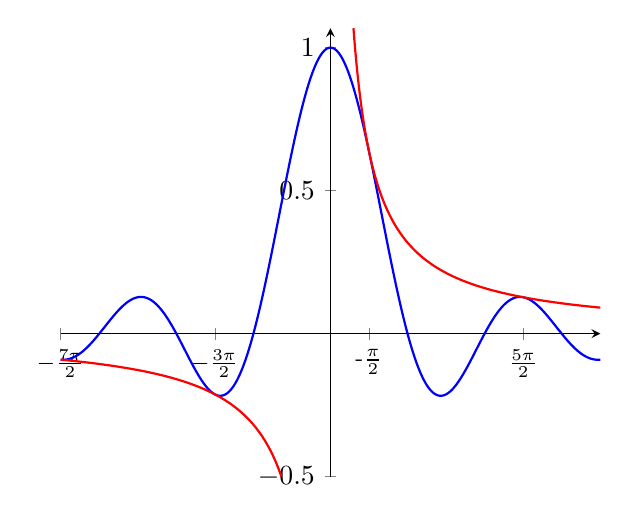
\begin{tikzpicture}
		\begin{axis}[axis x line=center,axis y line=center,restrict y to domain=-0.5:1.1,xmin=-11,xmax=11, xtick={-7*pi/2,-3*pi/2,pi/2,5*pi/2},xticklabel style={font=\footnotesize,fill=white},
		xticklabels={$-\frac{7\pi}{2}$,$-\frac{3\pi}{2}$,-$\frac{\pi}{2}$,$\frac{5\pi}{2}$},]
		\addplot[domain=-11:11,thick,blue, samples = 600] {sin(deg(x))/x};
		\addplot[domain=-11:11,thick,red, samples = 600] {1/x};
		\end{axis}
		\end{tikzpicture}
		\caption{Opgave~\ref{it:diff23}}
		\label{fig:diff23}
	\end{figure}
	
	
	
\end{enumerate}